% Provenance (never printed): see sources/outline_sources.md (Year 1: rigid plates on a
% sphere, Euler poles and angular velocities; relative velocities; triple junctions;
% finite rotations; the magnetic-anomaly timescale; satellite geodesy). Curves and maps
% from figdata/bachelor-1/euler_velocities.py, south_atlantic_fit.py and gpts_stripes.py;
% exercise and problem values in the Book 3 scratch calculator calc/ch12.py.
\chapter{Cinemática de placas sobre una esfera}\label{ch:b1:plate-kinematics}

Dos estaciones de posicionamiento por satélite llevan más de un cuarto de siglo registrando su posición cada día: una en Reikiavik,
al oeste de Islandia, la otra cerca de Stavanger, en la costa oeste de Noruega. La recta que las une, de \qty{1546}{km} de longitud,
crece \qty{17.5}{mm} cada año, casi dos centímetros. Nada en el terreno lo muestra; sin embargo, el fondo del Atlántico norte entre
las dos estaciones registra el mismo ensanchamiento a lo largo de millones de años: la lava erupcionada en la dorsal medioatlántica
adquirió la dirección del campo magnético terrestre al enfriarse, y el campo se ha invertido muchas veces, de modo que el fondo
oceánico lleva un registro en franjas de su propio crecimiento. Este capítulo convierte las placas de los años escolares en casquetes
rígidos sobre una esfera, describe sus movimientos con la geometría de las rotaciones, y muestra cómo el registro geológico y los
satélites miden los mismos movimientos.
% ledger: ngl:reyk, ngl:stas (chord lengthening computed in calc/ch12.py)

\begin{recall}
En una esfera, un \omterm{def:b1:spherical-astronomy:spherical-triangle}{círculo máximo} es la intersección con un plano que pasa por el centro, y un \omterm{def:b1:spherical-astronomy:spherical-triangle}{círculo menor} la de cualquier otro
plano; el teorema del coseno da la distancia angular entre dos puntos a partir de sus \omterm{def:b1:spherical-astronomy:geographic}{latitudes} y \omterm{def:b1:spherical-astronomy:geographic}{longitudes}, y el \omterm{def:b1:spherical-astronomy:horizontal}{acimut} de una
dirección se cuenta desde el norte hacia el este (\cref{ch:b1:spherical-astronomy}). Un cuerpo rígido que gira alrededor de un eje
fijo tiene una velocidad angular (física). La \omterm{def:b1:layered-earth:lithosphere}{litosfera} está rota en placas que se mueven unas respecto de otras a unos centímetros
al año, y el fondo oceánico lleva franjas magnéticas que registran las inversiones del campo magnético terrestre (libro 2, año 11).
\end{recall}

\section{Placas rígidas sobre una esfera}

Una placa cubre una gran parte de la esfera: la placa euroasiática se extiende desde el centro del Atlántico hasta el este de Siberia.
Su movimiento no puede describirse con una velocidad, como el de un coche; hay que describirlo con una rotación.

\begin{definition}[Placa rígida]\label{def:b1:plate-kinematics:rigid-plate}
Una \emph{placa rígida}\index{placa rígida} es una región de la \omterm{def:b1:layered-earth:lithosphere}{litosfera} cuyo interior no se deforma de forma medible: la distancia
entre dos cualesquiera de sus puntos permanece constante. El movimiento relativo de dos placas se absorbe a lo largo de su frontera
común, una zona estrecha de fallas, terremotos y volcanes.
\end{definition}

Ninguna placa es perfectamente rígida: las fronteras son zonas de decenas a centenares de kilómetros de ancho, y los interiores se
deforman lentamente. La hipótesis es que estas desviaciones son pequeñas frente a los movimientos relativos; se comprueba por la
coherencia de cada resultado de este capítulo.

Una \omterm{def:b1:plate-kinematics:rigid-plate}{placa rígida} sobre la superficie de una esfera se mueve sin cambiar la distancia entre dos cualesquiera de sus puntos, y el centro
de la Tierra no se mueve. Tal movimiento se describe con una matriz $3\times3$ $R$ que conserva las longitudes, una matriz
\emph{ortogonal} ($R^{\mathsf T}R = I$), y que conserva la orientación del espacio, de modo que $\det R = 1$: un punto de vector de
posición $\vec r$ va a $R\vec r$.

\begin{theorem}[Teorema de la rotación de Euler]\label{thm:b1:plate-kinematics:euler}
Todo desplazamiento de una \omterm{def:b1:plate-kinematics:rigid-plate}{placa rígida} sobre la esfera es una rotación alrededor de un eje que pasa por el centro de la Tierra: existe
un vector unitario $\vec n$ con $R\vec n = \vec n$, y la placa gira alrededor de $\vec n$ un cierto ángulo.
\end{theorem}

\begin{proof}
Probamos que $1$ es un autovalor de $R$, es decir $\det(R - I) = 0$. Como $R R^{\mathsf T} = I$, tenemos $R - I = R(I - R^{\mathsf T})$,
así que
\[
  \det(R - I) = \det R\,\det\bigl((I - R)^{\mathsf T}\bigr) = \det(I - R),
\]
usando $\det R = 1$ y el hecho de que una matriz y su transpuesta tienen el mismo determinante. Para una matriz $3\times3$,
$\det(I - R) = (-1)^3\det(R - I) = -\det(R - I)$. Así que $\det(R - I) =
-\det(R - I)$, que es cero. Existe, por tanto, un vector unitario $\vec n$ con $R\vec n = \vec n$: los dos puntos donde la recta que
pasa por el centro a lo largo de $\vec n$ corta la superficie no se mueven. En el plano perpendicular a $\vec n$, $R$ conserva
longitudes y orientación: hace girar ese plano un cierto ángulo, y así gira toda la esfera alrededor de $\vec n$.
\end{proof}

Durante un intervalo de tiempo lo bastante corto para que el movimiento no cambie, la rotación avanza a ritmo constante, y el movimiento
de una placa respecto de otra es una velocidad angular alrededor de un eje fijo.

\begin{definition}[Polo de Euler; vector de Euler]\label{def:b1:plate-kinematics:euler-pole}
El movimiento de una placa B respecto de una placa A es una rotación alrededor de un eje que pasa por el centro de la Tierra. El
\emph{polo de Euler}\index{polo de Euler} del par es el punto donde este eje corta la superficie, elegido de modo que la rotación sea
antihoraria vista desde encima de él; el punto antípoda es el polo opuesto. El \emph{vector de Euler}\index{vector de Euler}
$\vec\omega_{BA}$ es la velocidad angular de B respecto de A: apunta desde el centro de la Tierra hacia el polo de Euler, y su longitud
$\omega$ es la velocidad de rotación.
\end{definition}

Un \omterm{def:b1:plate-kinematics:euler-pole}{vector de Euler} se da por la \omterm{def:b1:spherical-astronomy:geographic}{latitud} y la longitud de su polo y por su velocidad, habitualmente en grados por millón de años. El
movimiento de la placa euroasiática respecto de la placa norteamericana, promediado sobre los últimos \qty{3.16}{Myr} a partir de 453
velocidades de expansión medidas en las dorsales que los separan, tiene su polo en \ang{61.8}\,N, \ang{139.6}\,E, en el este de Siberia,
y la velocidad \qty{0.210}{\degree\per\Myr}. En radianes por año,
\[
  \omega = \frac{0.210\times\pi/180}{\num{e6}} = \qty{3.665e-9}{rad.yr^{-1}},
\]
una vuelta completa en \qty{1714}{\Myr}.
% ledger: morvel:eu-na, morvel:summary

\section{Velocidades relativas}

\begin{theorem}[Velocidad en una placa que gira]\label{thm:b1:plate-kinematics:velocity}
Si la placa B gira respecto de la placa A con el \omterm{def:b1:plate-kinematics:euler-pole}{vector de Euler} $\vec\omega$, un punto de B en el vector de posición $\vec r$ (desde el
centro de la Tierra) se mueve respecto de A con la velocidad
\[
  \vec v = \vec\omega\times\vec r .
\]
\end{theorem}

\begin{proof}
Sea $\Delta$ el ángulo entre $\vec\omega$ y $\vec r$. Al girar B, el punto describe un círculo alrededor del eje, de radio $R\sin\Delta$,
donde $R$ es el radio de la Tierra; a la velocidad angular $\omega$, su rapidez es $\omega R\sin\Delta$. Su velocidad es tangente a
ese círculo, así que perpendicular al eje y al radio $\vec r$, y como la rotación es antihoraria alrededor de $\vec\omega$, su sentido es
el de $\vec\omega\times\vec r$. El vector $\vec\omega\times\vec r$ tiene precisamente esta dirección y sentido y la longitud
$\omega R\sin\Delta$.
\end{proof}

El ángulo $\Delta$ es la distancia angular entre el \omterm{def:b1:plate-kinematics:euler-pole}{polo de Euler} y el punto, que da el teorema del coseno a partir de \omterm{def:b1:spherical-astronomy:geographic}{latitudes} y
longitudes.

\begin{proposition}[Velocidad y dirección del movimiento relativo]\label{prop:b1:plate-kinematics:speed}
Sea el \omterm{def:b1:plate-kinematics:euler-pole}{polo de Euler} a \omterm{def:b1:spherical-astronomy:geographic}{latitud} $\varphi_p$ y \omterm{def:b1:spherical-astronomy:geographic}{longitud} $\lambda_p$, y el punto a $\varphi$ y $\lambda$. Entonces
\begin{enumerate}
  \item la distancia angular $\Delta$ del polo al punto cumple
        $\cos\Delta = \sin\varphi_p\sin\varphi + \cos\varphi_p\cos\varphi
        \cos(\lambda - \lambda_p)$;
  \item la velocidad relativa es $v = \omega R\sin\Delta$: nula en el polo, máxima,
        $\omega R$, sobre el \omterm{def:b1:spherical-astronomy:spherical-triangle}{círculo máximo} a \ang{90} de él;
  \item la dirección del movimiento es perpendicular al \omterm{def:b1:spherical-astronomy:spherical-triangle}{círculo máximo} que une el punto
        con el polo: su \omterm{def:b1:spherical-astronomy:horizontal}{acimut} es el del polo, visto desde el punto, más \ang{90}.
\end{enumerate}
\end{proposition}

\begin{proof}
(1) es el teorema del coseno en el \omterm{def:b1:spherical-astronomy:spherical-triangle}{triángulo esférico} formado por el polo norte geográfico, el \omterm{def:b1:plate-kinematics:euler-pole}{polo de Euler} y el punto, cuyos lados
desde el polo norte son $\ang{90} - \varphi_p$ y $\ang{90} - \varphi$, con el ángulo $\lambda - \lambda_p$ entre ellos. (2) se sigue del
teorema. (3) La velocidad es perpendicular a $\vec\omega$ y a $\vec r$, es decir, al plano que los contiene, el plano del \omterm{def:b1:spherical-astronomy:spherical-triangle}{círculo máximo}
que pasa por el punto y el polo. En el plano horizontal del punto es, por tanto, perpendicular a la dirección del polo; como la rotación
es antihoraria vista desde encima del polo, un punto se mueve a la derecha de la dirección en que ve el polo, lo que suma \ang{90} al
\omterm{def:b1:spherical-astronomy:horizontal}{acimut}.
\end{proof}

\begin{omfigure}
\begin{tikzpicture}[x=2.5cm, y=2.5cm, font=\scriptsize, >=Stealth]
% orthographic view from 20 deg above the "Euler equator": a point at polar angle D,
% longitude p about the pole projects to X = sin D sin p, Y = cos D cos 20 - sin D cos p sin 20;
% it is visible when cos p >= -cot D tan 20 (limits computed by hand: 129.08, 102.13, 90, 77.87)
\fill[omSea!12] (0,0) circle (1);
\draw[thick] (0,0) circle (1);
\foreach \D/\m in {30/129.08, 60/102.13, 90/90, 120/77.87} {
  \draw[blue!45!black, domain=-\m:\m, samples=60, variable=\p]
    plot ({sin(\D)*sin(\p)}, {cos(\D)*cos(20) - sin(\D)*cos(\p)*sin(20)});
  \draw[blue!45!black, densely dashed, domain=\m:360-\m, samples=60, variable=\p]
    plot ({sin(\D)*sin(\p)}, {cos(\D)*cos(20) - sin(\D)*cos(\p)*sin(20)});
}
\draw[densely dashed] (0,0) -- (0,0.9397);
\draw[->, very thick] (0,0.9397) -- (0,1.38) node[above] {$\vec\omega$};
\fill (0,0.9397) circle (0.9pt) node[anchor=south west] {polo de Euler};
\fill (0,0) circle (0.7pt);
% velocity arrows at longitude -35 deg about the pole, length 0.5 sin D
\draw[->, very thick, red!75!black] (-0.287,0.6737) -- ++(0.243,-0.058);
\draw[->, very thick, red!75!black] (-0.497,0.2272) -- ++(0.421,-0.101);
\draw[->, very thick, red!75!black] (-0.574,-0.2802) -- ++(0.487,-0.117);
\draw[->, very thick, red!75!black] (-0.497,-0.7124) -- ++(0.421,-0.101);
\draw[->] (0,0) -- (-0.497,0.2272) node[pos=0.55, below] {$\vec r$};
\draw (0,0.22) arc[start angle=90, end angle=155.4, radius=0.22];
\node at (-0.11,0.33) {$\Delta$};
\node[anchor=west] at (0.62,0.81) {$\Delta = \ang{30}$};
\node[anchor=west] at (0.88,0.47) {$\Delta = \ang{60}$};
\node[anchor=west] at (1.02,0.0) {$\Delta = \ang{90}$};
\node[anchor=west] at (0.88,-0.47) {$\Delta = \ang{120}$};
\end{tikzpicture}

\par\smallskip{\small Una placa que gira alrededor de su \omterm{def:b1:plate-kinematics:euler-pole}{polo de Euler}, vista desde un poco por encima del círculo a \ang{90} del polo.
Cada punto se mueve a lo largo de un \omterm{def:b1:spherical-astronomy:spherical-triangle}{círculo menor} alrededor del polo (las partes ocultas en discontinuo); su velocidad, mostrada por
las flechas rojas, es $\omega R\sin\Delta$, donde $\Delta$ es su distancia angular al polo: nula en el polo, máxima a \ang{90} de él.}
\label{fig:b1:plate-kinematics:euler-pole}
\end{omfigure}

La velocidad del movimiento relativo cambia, pues, a lo largo de una frontera de placas aunque las dos placas sean perfectamente
rígidas, y la dirección del movimiento gira con ella. Dos consecuencias dan forma a todo mapa de fronteras de placas.

\begin{proposition}[Las transformantes siguen círculos menores]\label{prop:b1:plate-kinematics:transforms}
Una falla transformante, a lo largo de la cual dos placas se deslizan una junto a otra sin abrirse ni cerrarse, yace sobre un \omterm{def:b1:spherical-astronomy:spherical-triangle}{círculo
menor} alrededor del \omterm{def:b1:plate-kinematics:euler-pole}{polo de Euler} de las dos placas. La dirección de expansión en una dorsal, y de convergencia en una zona de
subducción, también sigue esos \omterm{def:b1:spherical-astronomy:spherical-triangle}{círculos menores}.
\end{proposition}

\begin{proof}
En una falla transformante la velocidad relativa es paralela a la falla en cada punto. La velocidad relativa es en todas partes tangente
a los \omterm{def:b1:spherical-astronomy:spherical-triangle}{círculos menores} alrededor del polo (\cref{thm:b1:plate-kinematics:velocity}); una curva tangente en cada uno de sus puntos al
\omterm{def:b1:spherical-astronomy:spherical-triangle}{círculo menor} que pasa por ese punto es uno de esos círculos. La segunda afirmación es la tercera parte de
\cref{prop:b1:plate-kinematics:speed}.
\end{proof}

La dorsal medioatlántica entre Eurasia y Norteamérica es una escalera de segmentos de dorsal desplazados por fallas transformantes; las
transformantes se orientan cerca de los \omterm{def:b1:spherical-astronomy:horizontal}{acimutes} que predice el \omterm{def:b1:plate-kinematics:euler-pole}{vector de Euler}, y su orientación es uno de los datos que sirven para
localizar el polo. La velocidad de expansión a lo largo de la misma frontera crece con la distancia angular al polo:
\qtyrange{11}{12}{mm.yr^{-1}} en la dorsal de Gakkel, en el océano Ártico, cerca del polo, y \qty{23}{mm.yr^{-1}} justo al norte de las
Azores, a \ang{78} de él. La figura de abajo compara las velocidades que predice el \omterm{def:b1:plate-kinematics:euler-pole}{vector de Euler} a lo largo de toda la frontera con
las de un modelo de placas independiente.
% ledger: morvel:eu-na

\begin{method}[La velocidad en un punto]\label{met:b1:plate-kinematics:velocity}
\begin{enumerate}
  \item Conviértase la velocidad del \omterm{def:b1:plate-kinematics:euler-pole}{vector de Euler} a radianes por año y calcúlese
        $\omega R$, en \unit{mm.yr^{-1}} con $R = \qty{6371}{km}$.
  \item Calcúlese la distancia angular $\Delta$ del polo al punto con el teorema del coseno; la velocidad es $\omega R\sin\Delta$.
  \item Calcúlese el \omterm{def:b1:spherical-astronomy:horizontal}{acimut} $\beta$ del polo visto desde el punto, con
        $\tan\beta = \sin(\lambda_p - \lambda)\cos\varphi_p /
        \bigl(\cos\varphi\sin\varphi_p - \sin\varphi\cos\varphi_p
        \cos(\lambda_p - \lambda)\bigr)$ y el cuadrante del numerador y
        del denominador; el movimiento va hacia $\beta + \ang{90}$.
  \item Compruébese el sentido: el movimiento es el de la segunda placa respecto de la primera. Intercambiar las placas lo invierte.
\end{enumerate}
\end{method}

\begin{example}[Eurasia se aleja de Norteamérica en Islandia]\label{ex:b1:plate-kinematics:iceland}
Tómese el centro de Islandia a \ang{64.5}\,N, \ang{18}\,W, y el \omterm{def:b1:plate-kinematics:euler-pole}{vector de Euler} de Eurasia respecto de Norteamérica dado arriba.
Entonces $\omega R =
\num{3.665e-9}\times\qty{6.371e9}{mm} = \qty{23.35}{mm.yr^{-1}}$, y
\[
  \cos\Delta = \sin\ang{61.8}\sin\ang{64.5}
  + \cos\ang{61.8}\cos\ang{64.5}\cos(\ang{-18} - \ang{139.6}) = 0.60736,
\]
así que $\Delta = \ang{52.60}$ y $v = 23.35\sin\ang{52.60} = \qty{18.55}{mm.yr^{-1}}$.
El polo se ve con el \omterm{def:b1:spherical-astronomy:horizontal}{acimut} $\beta = \ang{13.1}$, algo al este del norte, sobre el Ártico; Eurasia se mueve hacia $\ang{103.1}$, este-sureste, es decir
\qty{18.07}{mm.yr^{-1}} hacia el este y \qty{4.20}{mm.yr^{-1}} hacia el sur.
% computed in calc/ch12.py and figdata/bachelor-1/euler_velocities.py
\end{example}

\begin{omfigure}
\begin{tikzpicture}
\begin{axis}[omrecord, width=0.84\linewidth, height=6.4cm, xmin=0, xmax=90, ymin=0, ymax=26,
  xtick={0,15,...,90}, xlabel={distancia angular al polo de Euler, $\Delta$ (grados)},
  ylabel={velocidad de expansión (\unit{mm.yr^{-1}})},
  legend style={font=\scriptsize, at={(0.99,0.03)}, anchor=south east, draw=none, fill=white, fill opacity=0.85, text opacity=1},
  legend cell align=left]
% computed in figdata/bachelor-1/euler_velocities.py
\addplot[only marks, mark=*, mark size=0.9pt, black!55] table[x=delta, y=pb2002] {figdata/out/bachelor-1-euler_velocities-mar.dat};
\addlegendentry{modelo de frontera PB2002, en cada paso de la frontera}
\addplot[only marks, mark=x, mark size=1.1pt, blue!60!black] table[x=delta, y=gps] {figdata/out/bachelor-1-euler_velocities-mar.dat};
\addlegendentry{vector de Euler por posicionamiento por satélite}
\addplot[very thick, red!75!black] table[x=delta, y=v] {figdata/out/bachelor-1-euler_velocities-curve.dat};
\addlegendentry{$\omega R\sin\Delta$, vector de Euler geológico}
\node[font=\scriptsize, anchor=south east] at (axis cs:52.6,19.6) {Islandia};
\draw[black!70] (axis cs:52.6,18.55) circle (2.5pt);
\node[font=\scriptsize, anchor=south] at (axis cs:78.4,23.6) {Azores};
\draw[black!70] (axis cs:78.4,22.87) circle (2.5pt);
\node[font=\scriptsize, anchor=south] (gk) at (axis cs:9,12) {dorsal de Gakkel};
\draw[black!70, -{Stealth[length=3pt]}] (gk.south) -- (axis cs:16.5,7.2);
\end{axis}
\end{tikzpicture}

\par\smallskip{\small Velocidades de expansión entre Eurasia y Norteamérica, desde el océano Ártico hasta las Azores, frente a la
distancia angular al \omterm{def:b1:plate-kinematics:euler-pole}{polo de Euler}. Rojo: el \omterm{def:b1:plate-kinematics:euler-pole}{vector de Euler} geológico (polo \ang{61.8}\,N, \ang{139.6}\,E,
\qty{0.210}{\degree\per\Myr}), que sitúa todas las velocidades sobre una misma curva seno. Gris: las velocidades de un modelo
independiente de frontera de placas en cada uno de sus pasos; difieren de la curva en un \qty{1}{\percent} de media. Azul: las
velocidades predichas en los mismos pasos por un \omterm{def:b1:plate-kinematics:euler-pole}{vector de Euler} calculado a partir del posicionamiento por satélite en el interior
de las dos placas (polo \ang{74.2}\,N, \ang{134.1}\,E, \qty{0.237}{\degree\per\Myr}): al estar su polo en otro lugar, sus velocidades
no están sobre la curva roja. Están a menos de una décima de las velocidades geológicas desde las Azores hasta Islandia, y mucho más
bajas en el Ártico, donde las velocidades son pequeñas y dependen mucho de la posición exacta del polo.}
\label{fig:b1:plate-kinematics:mar-rates}
\end{omfigure}
% ledger: morvel:eu-na, morvel:gps-eu-na, data:pb2002 (mean difference 0.96 per cent, euler_velocities.py)

\section{Composición de movimientos; uniones triples}

Las velocidades relativas se suman como las velocidades de la mecánica: si B se mueve respecto de A y C respecto de B, entonces C se
mueve respecto de A con la suma de las dos velocidades.

\begin{proposition}[Los vectores de Euler se suman]\label{prop:b1:plate-kinematics:addition}
Para tres placas A, B, C,
\[
  \vec\omega_{CA} = \vec\omega_{CB} + \vec\omega_{BA}, \qquad
  \vec\omega_{AB} = -\vec\omega_{BA}.
\]
\end{proposition}

\begin{proof}
En cada punto $\vec r$, $\vec v_{CA} = \vec v_{CB} + \vec v_{BA}$, es decir
$\vec\omega_{CA}\times\vec r = \vec\omega_{CB}\times\vec r +
\vec\omega_{BA}\times\vec r = (\vec\omega_{CB} + \vec\omega_{BA})\times\vec r$
por la linealidad del producto vectorial. Un vector $\vec u$ con
$\vec u\times\vec r = \vec 0$ para todo $\vec r$ es nulo, así que los dos \omterm{def:b1:plate-kinematics:euler-pole}{vectores de Euler}
son iguales. Intercambiar A y B invierte cada velocidad.
\end{proof}

Para sumar \omterm{def:b1:plate-kinematics:euler-pole}{vectores de Euler}, escríbase cada uno en componentes cartesianas, como sigue: $\omega(\cos\varphi_p
\cos\lambda_p, \cos\varphi_p\sin\lambda_p, \sin\varphi_p)$, súmense las componentes, y vuélvase a un polo y una velocidad. Los polos no
pueden sumarse; los \omterm{def:b1:plate-kinematics:euler-pole}{vectores de Euler} sí. La relación es una restricción potente. El movimiento de la placa nubia (África) respecto de
Eurasia es lento, y el registro geológico da pocas medidas directas: entre las Azores y Gibraltar, las únicas son los \omterm{def:b1:spherical-astronomy:horizontal}{acimutes} de una
sola transformante, la falla de Gloria. Se deduce en cambio de los dos movimientos de expansión, bien medidos, a través del Atlántico:
con $\vec\omega_{\mathrm{NB\,NA}}$ (polo
\ang{79.2}\,N, \ang{40.2}\,E, \qty{0.233}{\degree\per\Myr}) y
$\vec\omega_{\mathrm{EU\,NA}}$ de arriba, $\vec\omega_{\mathrm{NB\,EU}} =
\vec\omega_{\mathrm{NB\,NA}} - \vec\omega_{\mathrm{EU\,NA}}$ tiene su polo en
\ang{20.9}\,N, \ang{18.3}\,W, frente a África occidental, y la velocidad
\qty{0.123}{\degree\per\Myr} (\cref{exo:b1:plate-kinematics:7}).
% ledger: morvel:nb-na, morvel:eu-na, morvel:nb-eu

\begin{definition}[Unión triple; unión triple estable]\label{def:b1:plate-kinematics:triple-junction}
Una \emph{unión triple}\index{unión triple} es un punto donde se encuentran tres placas, y con ellas tres fronteras de placas, cada una
una dorsal (R), una fosa (T) o una falla transformante (F). Una unión triple es \emph{estable}\index{unión triple estable} si, al moverse las placas, conserva la misma geometría: los mismos tres tipos de frontera que se encuentran en los mismos ángulos.
\end{definition}

Cada frontera permite que la unión se mueva solo de ciertas maneras sin cambiar su geometría. Una dorsal simétrica se mantiene a medio
camino entre sus dos placas; una transformante conserva su orientación sea cual sea lo que haga la unión a lo largo de ella; una fosa
está fija a su placa cabalgante. La cuestión es si un único movimiento de la unión satisface las tres fronteras a la vez. Se responde
en el \emph{espacio de velocidades}: un diagrama en el que cada placa es un punto cuyo vector de posición es la velocidad de la placa
en la unión, respecto de cualquiera de las placas, de modo que el lado que une dos puntos es la velocidad relativa de las dos placas.

\begin{proposition}[Las uniones de tres dorsales son estables]\label{prop:b1:plate-kinematics:rrr}
Una unión de tres dorsales, cada una en expansión simétrica y perpendicular a su eje, es estable sean cuales sean las velocidades
relativas de las tres placas.
\end{proposition}

\begin{proof}
Sean $a$, $b$, $c$ los puntos de las tres placas en el espacio de velocidades. Una dorsal entre A y B que se expande simétricamente se
mueve a la velocidad media de sus dos placas, $(a + b)/2$, más cualquier velocidad a lo largo de su propio eje, que es perpendicular a
$ab$: las velocidades de la unión que dejan la dorsal sin cambios forman la mediatriz perpendicular del lado $ab$. La unión conserva su
geometría si su velocidad yace sobre las tres mediatrices a la vez. Las tres mediatrices de un triángulo siempre se cortan en un punto,
el centro de su círculo circunscrito. Así pues, siempre existe una velocidad de la unión.
\end{proof}

McKenzie y Morgan, que introdujeron en 1969 la distinción entre uniones estables e inestables, analizaron las combinaciones de este modo.
Una transformante permite que la unión se mueva solo a lo largo de sí misma, es decir, a lo largo de la recta que pasa por los puntos de
sus dos placas: una unión de tres transformantes nunca es, por tanto, estable, ya que las tres rectas que pasan por los lados de un
triángulo no tienen ningún punto en común. Para los demás tipos, la estabilidad impone condiciones sobre la orientación de las fronteras
y sobre las velocidades relativas.
% ledger: mckenzie:triple-junctions

\begin{omfigure}
\begin{tikzpicture}[font=\scriptsize, >=Stealth]
% (a) map view of an RRR junction, ridges perpendicular to the sides of the
% velocity triangle in (b): ray directions 110.6, -121.0, -10.8 degrees
\begin{scope}[x=1cm, y=1cm]
  \node[font=\small] at (0,2.25) {(a) mapa};
  \fill[omSea!12] (-2.4,-2.0) rectangle (2.4,2.0);
  \draw[ridge] (0,0) -- (110.6:2.0);
  \draw[ridge] (0,0) -- (-121.0:2.1);
  \draw[ridge] (0,0) -- (-10.8:2.3);
  \fill (0,0) circle (1.5pt) node[anchor=south west] {J};
  \node[font=\normalsize] at (-1.5,0.3) {A};
  \node[font=\normalsize] at (1.4,1.1) {B};
  \node[font=\normalsize] at (0.7,-1.4) {C};
  \draw[->, thick] ($(110.6:1.3)+(20.6:0.12)$) -- ++(20.6:0.45);
  \draw[->, thick] ($(110.6:1.3)+(200.6:0.12)$) -- ++(200.6:0.45);
  \draw[->, thick] ($(-121:1.3)+(-31:0.12)$) -- ++(-31:0.45);
  \draw[->, thick] ($(-121:1.3)+(149:0.12)$) -- ++(149:0.45);
  \draw[->, thick] ($(-10.8:1.5)+(-100.8:0.12)$) -- ++(-100.8:0.45);
  \draw[->, thick] ($(-10.8:1.5)+(79.2:0.12)$) -- ++(79.2:0.45);
\end{scope}
% (b) velocity space: a(0,0), b(2.4,0.9), c(2.0,-1.2); circumcentre (1.365, 0.009)
\begin{scope}[xshift=5.6cm, yshift=-0.2cm, x=1.25cm, y=1.25cm]
  \node[font=\small] at (1.2,1.95) {(b) espacio de velocidades};
  \draw[thick] (0,0) -- (2.4,0.9) -- (2.0,-1.2) -- cycle;
  \fill (0,0) circle (1.5pt) node[left] {$a$};
  \fill (2.4,0.9) circle (1.5pt) node[above right] {$b$};
  \fill (2.0,-1.2) circle (1.5pt) node[below right] {$c$};
  \draw[omRidge!80!black, densely dashed] ($(1.365,0.009)+(-0.351*1.4,0.936*1.4)$) -- ($(1.365,0.009)+(0.351*0.9,-0.936*0.9)$);
  \draw[omRidge!80!black, densely dashed] ($(1.365,0.009)+(0.982*1.5,-0.187*1.5)$) -- ($(1.365,0.009)+(-0.982*0.6,0.187*0.6)$);
  \draw[omRidge!80!black, densely dashed] ($(1.365,0.009)+(-0.514*1.6,-0.857*1.6)$) -- ($(1.365,0.009)+(0.514*0.6,0.857*0.6)$);
  \fill[omRidge!80!black] (1.365,0.009) circle (1.6pt);
  \node[anchor=north, omRidge!80!black] at (1.30,-0.05) {$j$};
  \node[anchor=south east] at (1.05,0.50) {$ab$};
\end{scope}
\end{tikzpicture}

\par\smallskip{\small Una unión J de tres dorsales entre las placas A, B y C.
(a) Mapa: cada dorsal (línea doble) se expande perpendicular a su eje (flechas).
(b) Espacio de velocidades: cada placa es un punto; el lado $ab$ es la velocidad de B
respecto de A, perpendicular a la dorsal entre ellas. Las velocidades de la unión que dejan
sin cambios una dorsal simétrica forman la mediatriz perpendicular del lado correspondiente (discontinua);
las tres mediatrices se cortan siempre, en $j$, la velocidad de la unión.}
\label{fig:b1:plate-kinematics:rrr}
\end{omfigure}

La \omterm{def:b1:plate-kinematics:triple-junction}{unión triple} de las Azores, hacia \ang{39.4}\,N, \ang{29.8}\,W, donde se encuentran las placas norteamericana, euroasiática y nubia,
es una unión de tres dorsales: la dorsal medioatlántica discurre al norte y al sur de ella, y el lento rift de Terceira
sale de ella hacia el este-sureste. En la unión, los dos \omterm{def:b1:plate-kinematics:euler-pole}{vectores de Euler} del par norteamericano dan a Eurasia \qty{22.9}{mm.yr^{-1}}
hacia \ang{95} y a Nubia \qty{19.2}{mm.yr^{-1}} hacia \ang{104}; Eurasia se aleja, pues, de Nubia a \qty{4.9}{mm.yr^{-1}} hacia
\ang{59}, una apertura este-nordeste--oeste-suroeste a través del rift de Terceira. La unión real no es un punto: la velocidad de
expansión a lo largo de la dorsal disminuye gradualmente, desde \qty{22.9}{mm.yr^{-1}} a \ang{40}\,N hasta \qty{19.8}{mm.yr^{-1}} a
\ang{38}\,N, a través de una pequeña placa de unos \qty{100}{km} de ancho atrapada entre las tres grandes: la microplaca de las Azores.
% ledger: morvel:azores, data:pb2002 (junction point at 39.40 N, 29.77 W, three spreading boundaries), morvel:nb-eu, morvel:eu-na, morvel:nb-na (velocities computed in calc/ch12.py)

\section{Rotaciones finitas}

El \omterm{def:b1:plate-kinematics:euler-pole}{vector de Euler} describe el movimiento actual, promediado sobre unos pocos millones de años. Para devolver las placas a donde
estaban hace mucho tiempo, hace falta la rotación que lleva una placa de su posición actual a su posición pasada.

\begin{definition}[Rotación finita]\label{def:b1:plate-kinematics:finite-rotation}
Una \emph{rotación finita}\index{rotación finita} es la rotación de la esfera, dada por un polo (\omterm{def:b1:spherical-astronomy:geographic}{latitud}, \omterm{def:b1:spherical-astronomy:geographic}{longitud}) y un ángulo, que
lleva una placa, o un trozo de su borde, de su posición actual a su posición en un tiempo dado respecto de otra placa. Un ángulo
positivo gira en sentido antihorario visto desde encima del polo.
\end{definition}

\begin{proposition}[Fórmula de Rodrigues]\label{prop:b1:plate-kinematics:rodrigues}
La rotación de ángulo $\alpha$ alrededor del vector unitario $\vec n$ lleva el
vector $\vec r$ a
\[
  \vec r\,' = \cos\alpha\,\vec r + (1 - \cos\alpha)(\vec n\cdot\vec r)\,\vec n
  + \sin\alpha\,\vec n\times\vec r .
\]
\end{proposition}

\begin{proof}
Descompóngase $\vec r$ en su parte a lo largo del eje, $\vec r_\parallel =
(\vec n\cdot\vec r)\vec n$, que la rotación no cambia, y en su parte perpendicular a ella, $\vec r_\perp = \vec r - \vec r_\parallel$. El vector
$\vec n\times\vec r = \vec n\times\vec r_\perp$ tiene la longitud de $\vec r_\perp$, es perpendicular a él y a $\vec n$, y está girado
\ang{90} en sentido antihorario respecto de él alrededor de $\vec n$. En el plano perpendicular a $\vec n$, la rotación de
ángulo $\alpha$ lleva $\vec r_\perp$ a $\cos\alpha\,\vec r_\perp +
\sin\alpha\,\vec n\times\vec r$. Sumando $\vec r_\parallel$ resulta $\vec r\,' =
\vec r_\parallel + \cos\alpha(\vec r - \vec r_\parallel) + \sin\alpha\,
\vec n\times\vec r$, que es la fórmula.
\end{proof}

La fórmula es lineal en $\vec r$; escrita con matrices, $\vec r\,' = R\vec r$
con
\[
  R = \cos\alpha\,I + (1 - \cos\alpha)\,\vec n\,\vec n^{\mathsf T}
  + \sin\alpha
  \begin{pmatrix} 0 & -n_z & n_y\\ n_z & 0 & -n_x\\ -n_y & n_x & 0\end{pmatrix},
\]
una matriz ortogonal de determinante $1$, como exige el teorema de Euler. Su traza
es $1 + 2\cos\alpha$, lo que da el ángulo de cualquier matriz de rotación
(\cref{exo:b1:plate-kinematics:10}).

Las \omterm{def:b1:plate-kinematics:finite-rotation}{rotaciones finitas} no conmutan. Si se gira el punto de \ang{0}\,N, \ang{0}\,E, situado sobre el eje $x$, \ang{90} alrededor del polo
norte, va a \ang{0}\,N, \ang{90}\,E, sobre el eje $y$; luego, \ang{90} alrededor del eje $x$, llega al polo norte. Hecho en el otro
orden, la primera rotación deja el punto donde está y la segunda lo lleva a \ang{0}\,N, \ang{90}\,E
(\cref{exo:b1:plate-kinematics:8}). Una sucesión de movimientos de placas debe componerse, por tanto, multiplicando las matrices en el
orden correcto, nunca sumando los ángulos; solo las velocidades angulares, que describen rotaciones infinitesimales, se suman como vectores.

\begin{omfigure}
\begin{tikzpicture}
\begin{axis}[axis equal image, width=0.8\linewidth, xmin=-85, xmax=55, ymin=-58, ymax=38,
  xtick={-80,-60,...,40}, ytick={-40,-20,0,20},
  xticklabel={$\pgfmathprintnumber{\tick}^\circ$}, yticklabel={$\pgfmathprintnumber{\tick}^\circ$},
  tick label style={font=\scriptsize}, axis background/.style={fill=omSea!10},
  unbounded coords=jump]
% computed in figdata/bachelor-1/south_atlantic_fit.py
\addplot[fill=omHypsLandC!60, draw=black!60, line width=0.3pt] table[x=lon, y=lat] {figdata/out/bachelor-1-south_atlantic_fit-af.dat};
\addplot[draw=black, line width=0.5pt] table[x=lon, y=lat] {figdata/out/bachelor-1-south_atlantic_fit-sa.dat};
\addplot[draw=blue!60!black, densely dashed, line width=0.6pt] table[x=lon, y=lat] {figdata/out/bachelor-1-south_atlantic_fit-sa84.dat};
\addplot[fill=red!40, fill opacity=0.55, draw=red!70!black, line width=0.5pt] table[x=lon, y=lat] {figdata/out/bachelor-1-south_atlantic_fit-sa120.dat};
\addplot[red!70!black, thick, densely dotted, -{Stealth}] table[x=lon, y=lat] {figdata/out/bachelor-1-south_atlantic_fit-track.dat};
\fill (axis cs:-34.9,-8.05) circle (1.6pt);
\node[font=\scriptsize, anchor=south east, fill=white, fill opacity=0.8, text opacity=1, inner sep=1pt] at (axis cs:-36,-7) {Recife};
  \node[font=\scriptsize, align=center] at (axis cs:-60,-17) {Sudamérica\\hoy};
\node[font=\scriptsize, blue!60!black, anchor=east] at (axis cs:-31,-46) {83.5 Ma};
\node[font=\scriptsize, red!60!black, fill=white, fill opacity=0.8, text opacity=1, inner sep=1pt] at (axis cs:-8,-22) {120.6 Ma};
  \node[font=\scriptsize] at (axis cs:22,12) {África};
\end{axis}
\end{tikzpicture}

\par\smallskip{\small Cierre del Atlántico Sur. Sudamérica (contorno negro) se lleva hacia atrás respecto de África mediante dos
\omterm{def:b1:plate-kinematics:finite-rotation}{rotaciones finitas} publicadas: a su posición a \qty{83.5}{Ma} (polo \ang{61.88}\,N, \ang{34.26}\,W, ángulo \ang{33.51}; discontinuo) y a
\qty{120.6}{Ma}, cuando el océano empezaba a abrirse (polo \ang{51.28}\,N, \ang{33.67}\,W, ángulo \ang{52.35}; rojo). La línea de puntos
es la trayectoria de Recife sobre su \omterm{def:b1:spherical-astronomy:spherical-triangle}{círculo menor} alrededor del polo más antiguo. La \omterm{def:b1:spherical-astronomy:geographic}{latitud} y la longitud se dibujan como una
cuadrícula cuadrada, que deforma las formas alejándolas del ecuador. Líneas de costa: Natural Earth.}
\label{fig:b1:plate-kinematics:south-atlantic}
\end{omfigure}
% ledger: heine:sam-saf, data:ne-land

El ajuste de las costas de Sudamérica y de África, notado desde hace mucho en los mapas, se convierte en un cálculo. Con la rotación de
\qty{120.6}{Ma}, la costa del noreste de Brasil cerca de Recife (\ang{8.05}\,S, \ang{34.9}\,W) llega a \ang{3.4}\,N, \ang{8.3}\,E, en la
costa del golfo de Guinea, tras un recorrido de unos \qty{5000}{km} a lo largo de su \omterm{def:b1:spherical-astronomy:spherical-triangle}{círculo menor}: una apertura media de unos
\qty{40}{mm.yr^{-1}}. El ajuste no es perfecto en todas partes: durante unos catorce millones de años antes de que se abriera el océano,
los dos continentes se estiraron lentamente alejándose, y una reconstrucción precisa debe restaurar primero los márgenes estirados y las
cuencas de rift a ambos lados.
% ledger: heine:sam-saf, heine:fit (Recife computed in south_atlantic_fit.py and calc/ch12.py)

\begin{history}[Tectónica sobre una esfera]
En 1965 Edward Bullard y dos colaboradores ajustaron por ordenador los continentes alrededor del Atlántico, con un criterio de mínimos
cuadrados: el mejor ajuste sigue la parte empinada del borde continental, a una profundidad de 500 brazas (unos \qty{900}{m}), y no la
línea de costa. El mismo año Tuzo Wilson describió una nueva clase de fallas, las fallas transformantes, y su relación con la deriva
continental. En 1967 Dan McKenzie y Robert Parker mostraron, con el Pacífico norte como ejemplo, que las zonas asísmicas de la
superficie se mueven como \omterm{def:b1:plate-kinematics:rigid-plate}{placas rígidas} sobre una esfera. En 1968 Jason Morgan describió la superficie como bloques corticales
limitados por dorsales, fosas y grandes fallas, y Xavier Le Pichon vinculó la expansión del fondo marino con la deriva continental. En
tres años, la deriva de los continentes se había convertido en la cinemática de casquetes rígidos sobre una esfera.
% ledger: bullard:fit, wilson:transform, mckenzie:sphere, morgan:blocks, lepichon:spreading
\end{history}

\section{Medición de los movimientos de placas}

\subsection*{El registro magnético del fondo oceánico}

La lava erupcionada en una dorsal adquiere, al enfriarse, una imantación en la dirección del campo terrestre en ese momento, y la
conserva al alejarse de la dorsal. Como el campo se invierte a intervalos irregulares, el fondo oceánico queda imantado en direcciones
alternadas, en bandas paralelas a la dorsal.

\begin{definition}[Anomalía magnética marina; cron de polaridad; escala de tiempo de polaridad]\label{def:b1:plate-kinematics:magnetic-anomaly}
Una \emph{anomalía magnética marina}\index{anomalía magnética marina} es la diferencia entre la intensidad del campo magnético medida en
el mar y la intensidad de un modelo de referencia del campo principal de la Tierra en el mismo lugar: es positiva sobre una \omterm{def:b1:layered-earth:layers}{corteza}
imantada en la dirección del campo actual, y negativa sobre una \omterm{def:b1:layered-earth:layers}{corteza} imantada en la dirección opuesta. Un \emph{cron de
polaridad}\index{cron de polaridad} es un intervalo de tiempo durante el cual el campo conservó una polaridad, designada por un número y
la letra n (normal, como hoy) o r (invertida). La \emph{escala de tiempo de polaridad geomagnética}\index{escala de tiempo de polaridad geomagnética} es la sucesión de crones de polaridad con las edades de sus límites.
\end{definition}

La escala de tiempo se construye datando las secuencias de inversiones en tierra y en testigos de sedimento marino profundo, y
ajustando el patrón de las anomalías del fondo oceánico, cuyos anchos conservan las duraciones relativas de los crones. El cron normal
actual, C1n, comenzó hace \qty{0.781}{Ma}, y el campo se ha invertido a intervalos irregulares: la escala cuenta veinticinco intervalos
normales en los últimos once millones de años, algunos de más de un millón de años, otros de poco más de diez mil años. La figura de
abajo muestra esa historia, hasta el final del cron C5n, y las franjas que escribe en el fondo de una dorsal lenta y en el de una rápida.
% ledger: iodp:gpts2004

\begin{omfigure}
\begin{tikzpicture}
\begin{axis}[name=gpts, width=0.9\linewidth, height=2.3cm, xmin=0, xmax=11.04, ymin=0, ymax=1,
  ytick=\empty, xtick={0,1,...,11}, tick label style={font=\scriptsize}, axis on top,
  xlabel={edad (Ma)}, label style={font=\scriptsize}, title={(a) escala de polaridad, \qtyrange{0}{11}{Ma}},
  title style={font=\small, yshift=-1.5ex}]
% computed in figdata/bachelor-1/gpts_stripes.py
\addplot[const plot, fill=black, draw=none] table[x=age, y=pol] {figdata/out/bachelor-1-gpts_stripes-gpts.dat} \closedcycle;
\node[font=\scriptsize, fill=white, inner sep=1pt] at (axis cs:0.39,0.5) {C1n};
\node[font=\scriptsize, fill=white, inner sep=1pt] at (axis cs:3.1,0.5) {C2An};
\node[font=\scriptsize, fill=white, inner sep=1pt] at (axis cs:4.75,0.5) {C3n};
\node[font=\scriptsize, fill=white, inner sep=1pt] at (axis cs:10.42,0.5) {C5n};
\end{axis}
\begin{axis}[name=slow, at={(gpts.south west)}, anchor=north west, yshift=-1.75cm, width=0.9\linewidth,
  height=2.3cm, xmin=-110.4, xmax=110.4, ymin=0, ymax=1, ytick=\empty, xtick={-100,-50,0,50,100},
  tick label style={font=\scriptsize}, axis on top, xlabel={distancia al eje de la dorsal (km)},
  label style={font=\scriptsize}, title={(b) velocidad de expansión por flanco \qty{10}{mm.yr^{-1}}},
  title style={font=\small, yshift=-1.5ex}]
\addplot[const plot, fill=black, draw=none] table[x=x, y=pol] {figdata/out/bachelor-1-gpts_stripes-stripes10.dat} \closedcycle;
\draw[red!80!black, very thick] (axis cs:0,0) -- (axis cs:0,1);
\end{axis}
\begin{axis}[at={(slow.south west)}, anchor=north west, yshift=-1.75cm, width=0.9\linewidth,
  height=2.3cm, xmin=-441.6, xmax=441.6, ymin=0, ymax=1, ytick=\empty, xtick={-400,-200,0,200,400},
  tick label style={font=\scriptsize}, axis on top, xlabel={distancia al eje de la dorsal (km)},
  label style={font=\scriptsize}, title={(c) velocidad de expansión por flanco \qty{40}{mm.yr^{-1}}},
  title style={font=\small, yshift=-1.5ex}]
\addplot[const plot, fill=black, draw=none] table[x=x, y=pol] {figdata/out/bachelor-1-gpts_stripes-stripes40.dat} \closedcycle;
\draw[red!80!black, very thick] (axis cs:0,0) -- (axis cs:0,1);
\end{axis}
\end{tikzpicture}

\par\smallskip{\small (a) La \omterm{def:b1:plate-kinematics:magnetic-anomaly}{escala de tiempo de polaridad geomagnética} a lo largo de los últimos \qty{11}{Myr} (negro: polaridad
normal, como hoy; blanco: invertida), con las edades de la escala de 2004, incluidos los subcrones cortos. (b) y (c) El fondo oceánico
que una dorsal (roja) construye durante el mismo tiempo, con expansión simétrica: cada intervalo de polaridad se convierte en un par de
franjas, una en cada flanco, de anchura igual a la velocidad de expansión por flanco multiplicada por su duración. A cuatro veces la
velocidad, el mismo patrón es cuatro veces más ancho; los eventos breves, como el Jaramillo (cerca de \qty{1}{Ma}), hacen que las franjas
sean de menos de un kilómetro de ancho en la dorsal lenta.}
\label{fig:b1:plate-kinematics:stripes}
\end{omfigure}

\begin{definition}[Velocidades de expansión media y total]\label{def:b1:plate-kinematics:spreading-rate}
En una dorsal, la \emph{velocidad de expansión media}\index{velocidad de expansión media} de un flanco es la velocidad a la que la
\omterm{def:b1:layered-earth:layers}{corteza} de ese flanco se aleja del eje de la dorsal. La \emph{velocidad de expansión total}\index{velocidad de expansión total} es la
velocidad a la que se separan las dos placas, la suma de las dos medias; es el doble de la media cuando la expansión es simétrica.
\end{definition}

\begin{method}[Una velocidad de expansión a partir de anomalías magnéticas]\label{met:b1:plate-kinematics:rate}
\begin{enumerate}
  \item En un perfil magnético perpendicular a la dorsal, identifíquese la sucesión de anomalías en ambos flancos por su patrón de
        franjas anchas y estrechas, y asígnese a la escala de tiempo de polaridad.
  \item Mídase la distancia desde el eje hasta el mismo límite de cron en cada flanco, y divídase por su edad: estas son las dos
        \omterm{def:b1:plate-kinematics:spreading-rate}{velocidades de expansión medias}, promediadas desde entonces. La velocidad total es su suma, o la distancia entre los dos límites
        dividida por la edad.
  \item Prefiérase un límite antiguo a uno joven: un error de un kilómetro en una distancia pesa menos sobre una distancia de cien
        kilómetros que sobre una de diez.
  \item Si el perfil no es perpendicular a la dorsal, proyéctense las distancias sobre la dirección de la expansión.
\end{enumerate}
\end{method}

El tercer punto no es solo cuestión de errores de lectura. La \omterm{def:b1:layered-earth:layers}{corteza} no adquiere su imantación a lo largo de una sola línea: la lava
fluye sobre la \omterm{def:b1:layered-earth:layers}{corteza} contigua, algo más antigua, los diques se intruyen en ella, y la \omterm{def:b1:layered-earth:layers}{corteza} inferior se imanta más tarde que la
superior. Todos estos procesos desplazan hacia fuera del eje los límites entre franjas, de modo que la distancia entre dos límites de
la misma edad supera la anchura de \omterm{def:b1:layered-earth:layers}{corteza} realmente formada. El desplazamiento total de los dos lados es de \qtyrange{1}{3}{km} como
máximo en la mayoría de las dorsales, y alcanza los \qty{5.0}{km} en la dorsal de Reykjanes. Las compilaciones cuidadosas corrigen las
velocidades a la baja por este desplazamiento hacia fuera, en \qtyrange{0.6}{2.6}{mm.yr^{-1}}, y las promedian durante los últimos
\qty{3.16}{Myr} en las dorsales lentas, hasta las anomalías del cron C2An, y durante \qty{0.78}{Myr} en las rápidas. En la dorsal de
Gakkel, escasa de magma, faltan las anomalías del subcron corto de Jaramillo y del cron C2n, mientras que en la dorsal de Reykjanes, al
sur de Islandia, que se expande a menos de \qty{20}{mm.yr^{-1}} pero con un abundante suministro de magma, están claramente reconocidas.
% ledger: morvel:summary, morvel:profiles, morvel:outward

\subsection*{Geodesia por satélite}

Desde los años 1990, las posiciones de las estaciones permanentes se miden cada día por posicionamiento por satélite. Una serie de
posiciones diarias durante diez años o más da la velocidad de una estación, una vez tratados los movimientos estacionales y los saltos
causados por terremotos o por cambios de equipo (\cref{exo:b1:plate-kinematics:12}).
% ledger: ngl:start, usgs:gps

\begin{inthefield}[Una estación permanente]
\begin{minipage}[t]{0.7\linewidth}\vspace{0pt}
Una estación permanente de posicionamiento por satélite es un instrumento tranquilo. La antena, bajo su cúpula impermeable, se apoya
sobre la cima de un pilar o de un mástil arriostrado anclado en la roca, de modo que se mueve con la \omterm{def:b1:layered-earth:layers}{corteza} y con nada más; el
receptor, en la base, registra de forma continua las señales de cada satélite a la vista y las envía a un centro de datos. Allí, los
analistas calculan una posición para cada día, en un sistema de referencia ligado a una red mundial de estaciones, y publican series
temporales y velocidades. La historia de una estación importa tanto como sus datos: cada cambio de antena o de receptor se registra,
porque puede desplazar la posición calculada.
\end{minipage}\hfill
\begin{minipage}[t]{0.26\linewidth}\vspace{0pt}
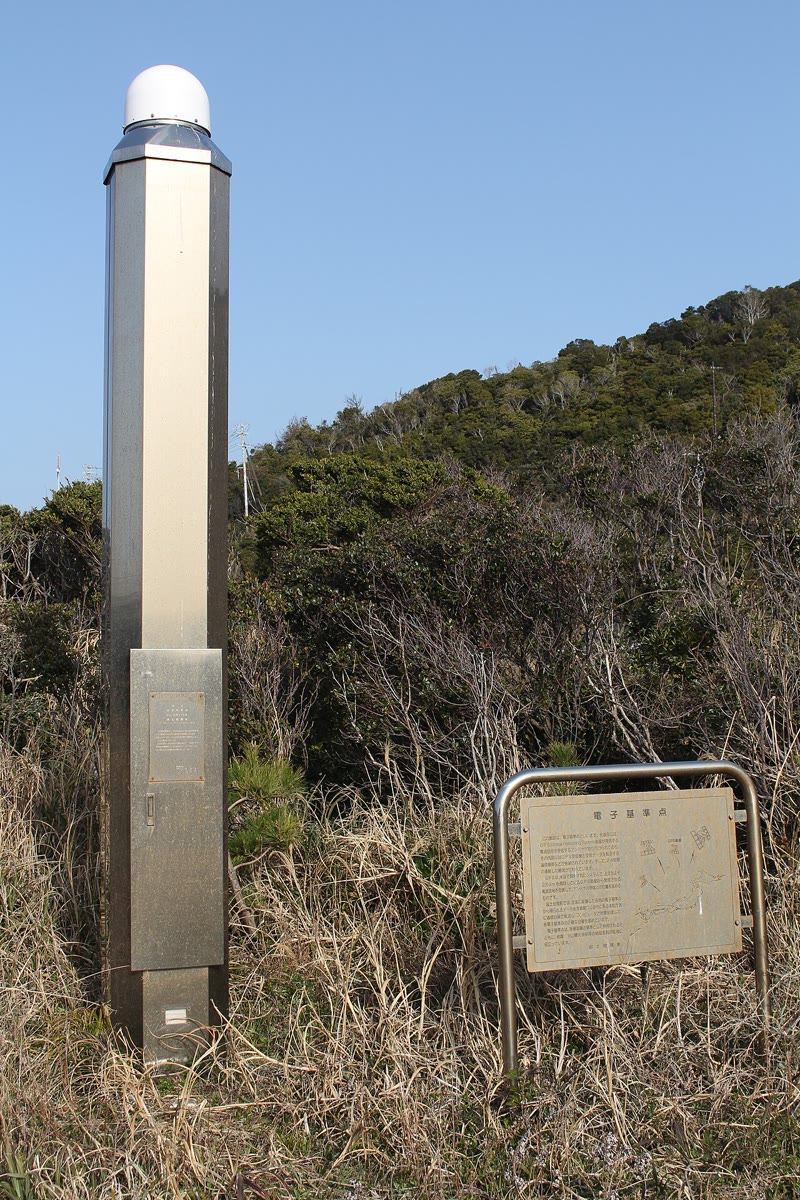
\includegraphics[width=\linewidth]{images/book3/b1-gnss-station.jpg}

{\scriptsize Una estación permanente en Japón, con su antena bajo la cúpula
(Alpsdake, CC BY-SA 4.0).}
\end{minipage}
\end{inthefield}

Las velocidades de las estaciones en el interior de dos placas dan un \omterm{def:b1:plate-kinematics:euler-pole}{vector de Euler} propio, independiente del registro geológico.
Para Eurasia respecto de Norteamérica, un vector así predice \qty{17.0}{mm.yr^{-1}} en Islandia, cerca de un \qty{8}{\percent} menos que
los \qty{18.6}{mm.yr^{-1}} promediados sobre \qty{3.16}{Myr} (figura de arriba). La recta entre Reikiavik y Stavanger, ambas en partes
estables de sus placas, se alarga \qty{17.5}{mm.yr^{-1}}; el vector de satélite predice \qty{17.1}{mm.yr^{-1}}, el geológico
\qty{18.6}{mm.yr^{-1}}. A través del Atlántico norte, una velocidad medida a lo largo de unas pocas décadas y una velocidad promediada
sobre tres millones de años concuerdan así dentro de una décima: allí, las placas se mueven hoy casi como se han movido durante
millones de años.
% ledger: morvel:gps-eu-na, morvel:eu-na, ngl:reyk, ngl:stas (chord rates computed in calc/ch12.py)

Dentro de la zona de frontera el cuadro es menos sencillo, porque las estaciones se mueven con más que las placas. Más de una décima
parte de Islandia yace bajo casquetes de hielo, y la mayoría de ellos pierden masa desde hacia 1890: la \omterm{def:b1:layered-earth:layers}{corteza} bajo ellos se eleva a
medida que disminuye la carga, y se mueve horizontalmente alejándose del hielo que adelgaza. La estación de Höfn, en la costa sureste
cerca del mayor casquete, se eleva \qty{12.9}{mm.yr^{-1}}.
% ledger: spaans:iceland-gia, ngl:hofn

\section{Ejercicios}

Tómese $R = \qty{6371}{km}$ en todo el capítulo.

\begin{exercise}[$\star$]\label{exo:b1:plate-kinematics:1}
El \omterm{def:b1:plate-kinematics:euler-pole}{vector de Euler} de Eurasia respecto de Norteamérica tiene la velocidad \qty{0.210}{\degree\per\Myr}. (a) Conviértase a
\unit{rad.yr^{-1}} y a \unit{rad.s^{-1}}. (b) ¿Cuánto tardaría una vuelta completa? (c) Calcúlese $\omega R$ en \unit{mm.yr^{-1}}.
% ledger: morvel:eu-na
\end{exercise}

\begin{exercise}[$\star$]\label{exo:b1:plate-kinematics:2}
Con el mismo \omterm{def:b1:plate-kinematics:euler-pole}{vector de Euler}, calcúlese la velocidad relativa de las dos placas a \ang{30}, \ang{60} y \ang{90} del \omterm{def:b1:plate-kinematics:euler-pole}{polo de Euler}.
¿Dónde a lo largo de la frontera de placas sería más rápida la expansión?
\end{exercise}

\begin{exercise}[$\star$]\label{exo:b1:plate-kinematics:3}
El subcron normal de Jaramillo duró desde \qty{1.072}{Ma} hasta \qty{0.988}{Ma}. (a) ¿Cuál es la anchura de la franja que forma en cada
flanco de una dorsal con una \omterm{def:b1:plate-kinematics:spreading-rate}{velocidad de expansión media} de \qty{50}{mm.yr^{-1}}? ¿Y de \qty{10}{mm.yr^{-1}}? (b) ¿Cuál es la anchura
total de la franja del cron normal actual, que comenzó hace \qty{0.781}{Ma}, en una dorsal con una velocidad media de
\qty{10}{mm.yr^{-1}}?
% ledger: iodp:gpts2004
\end{exercise}

\begin{exercise}[$\star$]\label{exo:b1:plate-kinematics:4}
En un perfil a través de una dorsal, el borde joven de la anomalía del cron C2An, de \qty{2.581}{Ma}, yace a \qty{66}{km} al oeste del eje
y a \qty{64}{km} al este de él. Calcúlense las dos \omterm{def:b1:plate-kinematics:spreading-rate}{velocidades de expansión medias} y la velocidad total. ¿Es simétrica la expansión?
% ledger: iodp:gpts2004
\end{exercise}

\begin{exercise}[$\star\star$]\label{exo:b1:plate-kinematics:5}
Un punto de la dorsal de Gakkel, en el océano Ártico, se sitúa en \ang{85}\,N, \ang{0}\,E. Calcúlese su distancia angular al \omterm{def:b1:plate-kinematics:euler-pole}{polo de
Euler} de Eurasia respecto de Norteamérica (\ang{61.8}\,N, \ang{139.6}\,E, \qty{0.210}{\degree\per\Myr}) y la velocidad de expansión
allí. Compárese con las velocidades medidas de \qtyrange{11}{12}{mm.yr^{-1}}.
% ledger: morvel:eu-na
\end{exercise}

\begin{exercise}[$\star\star$]\label{exo:b1:plate-kinematics:6}
En la \omterm{def:b1:plate-kinematics:triple-junction}{unión triple} de las Azores, en \ang{39.44}\,N, \ang{29.83}\,W, calcúlense (a) la distancia angular al \omterm{def:b1:plate-kinematics:euler-pole}{polo de Euler} de Eurasia
respecto de Norteamérica, (b) la velocidad de expansión y (c) el \omterm{def:b1:spherical-astronomy:horizontal}{acimut} del movimiento relativo. (d) ¿Qué orientación predice para las
fallas transformantes de la dorsal situada justo al norte de la unión?
% ledger: morvel:eu-na, morvel:azores
\end{exercise}

\begin{exercise}[$\star\star$]\label{exo:b1:plate-kinematics:7}
(a) Escríbanse en componentes cartesianas los \omterm{def:b1:plate-kinematics:euler-pole}{vectores de Euler} $\vec\omega_{\mathrm{EU\,NA}}$ (\ang{61.8}\,N, \ang{139.6}\,E,
\qty{0.210}{\degree\per\Myr}) y $\vec\omega_{\mathrm{NB\,NA}}$ (\ang{79.2}\,N, \ang{40.2}\,E, \qty{0.233}{\degree\per\Myr}), en
\unit{\degree\per\Myr}. (b) Dedúzcase $\vec\omega_{\mathrm{NB\,EU}}$, su polo y su velocidad. (c) ¿Por qué es esta la mejor manera
de conocer el movimiento de Nubia respecto de Eurasia?
% ledger: morvel:eu-na, morvel:nb-na
\end{exercise}

\begin{exercise}[$\star\star$]\label{exo:b1:plate-kinematics:8}
Sea $\vec e_x$ el vector hacia \ang{0}\,N, \ang{0}\,E, $\vec e_y$ hacia \ang{0}\,N, \ang{90}\,E y $\vec e_z$ hacia el polo norte. Con la
fórmula de Rodrigues, calcúlese la imagen de $\vec e_x$ (a) por la rotación de \ang{90} alrededor de $\vec e_z$ seguida de la rotación
de \ang{90} alrededor de $\vec e_x$; (b) por las mismas dos rotaciones en orden inverso. (c) ¿Qué significa esto para la
reconstrucción de las posiciones pasadas de una placa?
\end{exercise}

\begin{exercise}[$\star\star$]\label{exo:b1:plate-kinematics:9}
Tres placas A, B y C se encuentran en una unión de tres dorsales. Respecto de A, la placa B se mueve a \qty{30}{mm.yr^{-1}} hacia el este
y la placa C a \qty{40}{mm.yr^{-1}} hacia el sur. (a) Dibújese el triángulo de velocidades. (b) Calcúlese la velocidad y el \omterm{def:b1:spherical-astronomy:horizontal}{acimut} de C
respecto de B. (c) ¿Cuál es la orientación de la dorsal entre B y C si se expande perpendicular a su eje?
\end{exercise}

\begin{exercise}[$\star\star\star$]\label{exo:b1:plate-kinematics:10}
(a) Muéstrese que la traza de la matriz $R$ de una rotación de ángulo $\alpha$ alrededor de cualquier eje es $1 + 2\cos\alpha$. (b) La matriz
\[
  R = \begin{pmatrix} 0 & 0 & 1\\ 1 & 0 & 0\\ 0 & 1 & 0\end{pmatrix}
\]
es ortogonal con determinante $1$. Hállense su eje, como \omterm{def:b1:spherical-astronomy:geographic}{latitud} y \omterm{def:b1:spherical-astronomy:geographic}{longitud}, y su ángulo. (c) Compruébese la respuesta aplicando $R$ a
$\vec e_x$, $\vec e_y$ y $\vec e_z$.
\end{exercise}

\begin{exercise}[$\star\star\star$]\label{exo:b1:plate-kinematics:11}
Antes del posicionamiento por satélite, los \omterm{def:b1:plate-kinematics:euler-pole}{polos de Euler} se hallaban a partir de las orientaciones de las fallas transformantes. (a)
Muéstrese que el \omterm{def:b1:plate-kinematics:euler-pole}{polo de Euler} yace sobre el \omterm{def:b1:spherical-astronomy:spherical-triangle}{círculo máximo} que pasa por un punto de una falla transformante y es perpendicular a la
falla allí, y que por tanto el polo está en la dirección de $\vec t_1\times\vec t_2$, donde $\vec t_1$ y $\vec t_2$ son vectores unitarios
a lo largo de dos fallas transformantes de la misma frontera.
(b) Las fallas transformantes se orientan a \ang{95} cerca de la \omterm{def:b1:plate-kinematics:triple-junction}{unión triple} de las Azores (\ang{39.44}\,N, \ang{29.83}\,W) y a
\ang{103} en Islandia (\ang{64.5}\,N, \ang{18}\,W). El vector unitario horizontal en la \omterm{def:b1:spherical-astronomy:geographic}{latitud} $\varphi$ y \omterm{def:b1:spherical-astronomy:geographic}{longitud} $\lambda$ que apunta
hacia el \omterm{def:b1:spherical-astronomy:horizontal}{acimut} $\beta$ es $\sin\beta\,\vec e +
\cos\beta\,\vec n$, con $\vec e = (-\sin\lambda, \cos\lambda, 0)$ y $\vec n =
(-\sin\varphi\cos\lambda, -\sin\varphi\sin\lambda, \cos\varphi)$. Localícese el polo. (c) ¿Qué tan bien determinan dos transformantes el polo?
% ledger: morvel:eu-na
\end{exercise}

\begin{exercise}[$\star\star\star$]\label{exo:b1:plate-kinematics:12}
La posición hacia el este de una estación, cada tres meses durante tres años, es
(en milímetros, desde $t = 0$):
\begin{center}\small
\begin{tabular}{l*{13}{c}}
\hline
$t$ (yr) & 0 & 0.25 & 0.5 & 0.75 & 1 & 1.25 & 1.5 & 1.75 & 2 & 2.25 & 2.5 & 2.75 & 3\\
$x$ (mm) & 4 & 5 & 6 & 15 & 24 & 25 & 26 & 65 & 74 & 75 & 76 & 85 & 94\\
\hline
\end{tabular}
\end{center}
Se compone de un movimiento estable, de una oscilación estacional y de un salto causado por un terremoto. (a) Calcúlese la velocidad a
partir de las posiciones primera y última. (b) Calcúlense las nueve diferencias entre posiciones separadas exactamente un año, y su
mediana. (c) Explíquese por qué la mediana de las diferencias anuales es una estimación robusta de la velocidad estable, y cuándo fallaría.
\end{exercise}

\section{Problema: Islandia se separa}

\begin{problem}[{Problema de fin de semana --- la apertura del Atlántico norte a través de Islandia, medida de tres maneras}]
\label{pb:b1:plate-kinematics:1}
% values: calc/ch12.py (Part II profile invented for the problem; real Euler
% vectors, chron ages and station velocities)
% ledger: morvel:eu-na, morvel:nb-na, iodp:gpts2004, ngl:reyk, ngl:stas, ngl:hofn
Islandia se asienta sobre la dorsal medioatlántica, entre la placa norteamericana al oeste y la placa euroasiática al este. Tómese
$R = \qty{6371}{km}$ y, para Eurasia respecto de Norteamérica, el \omterm{def:b1:plate-kinematics:euler-pole}{vector de Euler} con su polo en \ang{61.8}\,N, \ang{139.6}\,E y la
velocidad \qty{0.210}{\degree\per\Myr}.

\medskip
\noindent\textbf{Parte I --- El vector de placa.}
\begin{enumerate}
  \item Conviértase la velocidad a \unit{rad.yr^{-1}} y calcúlese $\omega R$ en
        \unit{mm.yr^{-1}}.
  \item Calcúlese la distancia angular $\Delta$ del polo al centro de Islandia,
        \ang{64.5}\,N, \ang{18}\,W.
  \item Dedúzcase la \omterm{def:b1:plate-kinematics:spreading-rate}{velocidad de expansión total} a través de Islandia que predice el
        vector de placa.
  \item Calcúlese el \omterm{def:b1:spherical-astronomy:horizontal}{acimut} del polo visto desde Islandia, y el \omterm{def:b1:spherical-astronomy:horizontal}{acimut} del movimiento
        de Eurasia respecto de Norteamérica.
  \item Descompóngase esta velocidad en sus componentes hacia el este y hacia el norte.
  \item En la dorsal de Gakkel, a \ang{86}\,N, \ang{60}\,E, ¿qué velocidad da el mismo vector? ¿Por qué la frontera allí es tanto más lenta?
\end{enumerate}

\noindent\textbf{Parte II --- Las franjas magnéticas.}
Un perfil magnético de un barco a través de la dorsal de Reykjanes, al suroeste de Islandia hacia \ang{63}\,N, \ang{23}\,W, recorrido en la
dirección de expansión, da las siguientes distancias desde el eje a tres límites de crones (un perfil construido para este problema):
\begin{center}\small
\begin{tabular}{lccc}
\hline
límite & edad (Ma) & al oeste del eje (km) & al este del eje (km)\\
\hline
base de C1n & 0.781 & 9.7 & 10.1\\
borde joven de C2An & 2.581 & 26.8 & 27.3\\
borde joven de C5n & 9.779 & 94 & 97\\
\hline
\end{tabular}
\end{center}
\begin{enumerate}[resume]
  \item Desde el borde joven de C5n, calcúlense las dos \omterm{def:b1:plate-kinematics:spreading-rate}{velocidades de expansión medias}.
  \item Dedúzcase la \omterm{def:b1:plate-kinematics:spreading-rate}{velocidad de expansión total} desde \qty{9.8}{Ma}.
  \item Calcúlese también la velocidad total a partir de los dos límites más jóvenes. ¿Concuerdan las tres? Descríbase cómo cambian con
        la edad del límite.
  \item ¿Es simétrica la expansión? ¿Cambia la asimetría la velocidad total?
  \item En la dorsal de Reykjanes, los límites entre franjas están desplazados hacia fuera del eje \qty{5.0}{km} en total, en ambos
        flancos juntos. Corríjanse las tres velocidades totales. ¿Por qué la corrección importó más para el límite más joven?
  \item ¿Cuál es la anchura de la franja del subcron de Jaramillo (\qtyrange{1.072}{0.988}{Ma}) en cada flanco, con la velocidad media
        corregida? Compárese con el desplazamiento de la pregunta 11. La anomalía de Jaramillo se reconoce, no obstante, con claridad en
        los perfiles de la dorsal de Reykjanes, pero falta en la dorsal de Gakkel: ¿qué sugiere eso?
  \item El vector de placa predice \qty{19.0}{mm.yr^{-1}} en el perfil. Compárese con sus velocidades corregidas.
\end{enumerate}

\noindent\textbf{Parte III --- Los satélites.}
Las estaciones permanentes REYK (Reikiavik, \ang{64.139}\,N, \ang{21.955}\,W) y STAS (Stavanger, \ang{59.018}\,N, \ang{5.599}\,E) se sitúan
en las placas norteamericana y euroasiática. Sus velocidades medidas hacen que la recta entre ellas se alargue \qty{17.5}{mm.yr^{-1}}.
\begin{enumerate}[resume]
  \item Calcúlese la distancia angular entre las dos estaciones, y la longitud de la recta.
  \item ¿Cuánto tarda la recta en alargarse un metro?
  \item El vector de placa da a STAS una velocidad de \qty{18.9}{mm.yr^{-1}} hacia \ang{114.8} respecto de Norteamérica. El \omterm{def:b1:spherical-astronomy:spherical-triangle}{círculo máximo}
        desde REYK llega a STAS con \omterm{def:b1:geological-maps:attitude}{rumbo} a \ang{123.1}. Calcúlese la componente de la velocidad a lo largo de esta dirección, y después
        el alargamiento previsto de la recta, que forma el ángulo $\Delta/2$ con la horizontal en STAS.
  \item Compárense el alargamiento medido y el previsto. ¿Qué podría explicar la diferencia?
  \item Respecto de Norteamérica, REYK se mueve \qty{1.07}{mm.yr^{-1}} hacia el oeste y \qty{0.97}{mm.yr^{-1}} hacia el sur, y la
        estación HOFN (Höfn, sureste de Islandia) a \qty{21.12}{mm.yr^{-1}} hacia el este y \qty{6.97}{mm.yr^{-1}} hacia el sur.
        Calcúlense la velocidad y el \omterm{def:b1:spherical-astronomy:horizontal}{acimut} de HOFN respecto de REYK.
  \item Compárese con la Parte I. HOFN también se eleva \qty{12.9}{mm.yr^{-1}}. ¿Por qué las estaciones dentro de Islandia son una mala
        medida del movimiento de la placa?
\end{enumerate}

\noindent\textbf{Parte IV --- Diez millones de años, y la unión del sur.}
\begin{enumerate}[resume]
  \item En \qty{10}{Myr}, ¿qué ángulo gira Eurasia respecto de Norteamérica alrededor del polo?
  \item ¿Cuánto recorre un punto de Eurasia en el centro de Islandia a lo largo de su \omterm{def:b1:spherical-astronomy:spherical-triangle}{círculo menor} en ese tiempo? Compárese con la anchura
        corregida de la \omterm{def:b1:layered-earth:layers}{corteza} formada desde el borde joven de C5n en la Parte II.
  \item En la \omterm{def:b1:plate-kinematics:triple-junction}{unión triple} de las Azores, los vectores de placa dan a Eurasia \qty{22.9}{mm.yr^{-1}} hacia \ang{95.1} y a Nubia
        \qty{19.2}{mm.yr^{-1}} hacia \ang{103.8}, ambos respecto de Norteamérica. Calcúlese la velocidad de Eurasia respecto de Nubia.
  \item ¿Es estable esta unión? ¿Qué tipo de frontera implica entre Eurasia y Nubia la velocidad de la pregunta 22?
  \item Reúnanse las velocidades de apertura de las Partes I, II y III. ¿Cuáles concuerdan, y qué método mide el movimiento de las placas
        en el intervalo de tiempo más corto?
  \item Con precisión de milímetro por año, ¿qué \omterm{def:b1:plate-kinematics:spreading-rate}{velocidad de expansión total} a través de Islandia dan a la vez el vector de placa y las
        franjas magnéticas corregidas?
\end{enumerate}
\end{problem}
